\documentclass{rapportUmons}
\usepackage[nottoc]{tocbibind} % needed for displaying bibliography and other in the table of contents
\usepackage[ruled, linesnumbered, french]{algorithm2e}
\usepackage[utf8]{inputenc}
\usepackage[T1]{fontenc}
\usepackage[french]{babel}
\usepackage{graphicx}
\usepackage{subcaption}
\usepackage{listings}
\usepackage{hyperref}
\usepackage{booktabs}
\usepackage{amsmath}
\usepackage{xcolor}
\usepackage{csvsimple}
\usepackage[autostyle]{csquotes}
\usepackage[
    defernumbers=true,
    backend=biber,
    style=ieee
]{biblatex}
\addbibresource{book.bib}
\graphicspath{{./images/}}

\begin{document}

\begin{titlepage}

\newcommand{\HRule}{\rule{\linewidth}{0.5mm}}

\center 
%----------------------------------------------------------------------------------------
%	HEADING SECTIONS
%----------------------------------------------------------------------------------
\textsc{\LARGE}\\[1.5cm]

\vspace{3cm}

\textsc{\LARGE Université de Mons}\\[1.5cm]
\textsc{\LARGE Machine Learning }\\[0.5cm]
\textsc{\LARGE Rapport du projet}\\[0.5cm]

%----------------------------------------------------------------------------------------
%	TITLE SECTION
%----------------------------------------------------------------------------------------
\HRule \\ [0.4cm]
{\huge\bfseries Prédiction du score de Macron au 2nd tour des élections 2022}\\ [0.4cm]
\HRule \\ [1.5cm]
%----------------------------------------------------------------------------------------
%	AUTHOR SECTION
%----------------------------------------------------------------------------------------
\begin{minipage}{0.4\textwidth}
\begin{flushleft} \large
\emph{Étudiants:}\\
\textsc{Meyouguem Stela}\\
\textsc{Djamgoum Roland}\\
\textsc{Mebou Prestonne}\\


\end{flushleft}
\end{minipage}
~
\begin{minipage}{0.4\textwidth}
\begin{flushright}\large
\emph{Encadreur:} \\

Pr.  Pierre VANDENHOVE

\end{flushright}
\end{minipage}\\[2cm]


{\Large Année académique 2024-2025}\\[2cm]


\includegraphics[width=6cm]{images/umonslogo.png}\\[1cm]

\end{titlepage}

\pagenumbering{roman}

\tableofcontents

\newpage

\listoffigures 

\clearpage

\pagenumbering{arabic}





\section{Introduction}




Ce projet a pour objectif principal la mise en pratique des techniques de \textit{Machine Learning} dans le contexte suivant~: la prédiction du score électoral d'Emmanuel Macron au second tour de l'élection présidentielle française de 2022, à l'échelle de chaque commune de la France métropolitaine.
Nous voulons modéliser le pourcentage de voix obtenues par Emmanuel Macron, noté \% Voix/Ins, soit le nombre de voix exprimées pour Macron rapporté au nombre total d'inscrits, incluant les abstentionnistes et les votes nuls. Cette variable continue est modélisée à l'aide d'algorithmes de régression. Dans ce projet, nous utilisons ici deux modèles: la régression Lasso et XGBoost Regression.
Le jeu de données principal, \texttt{results\_train.csv}, regroupe les résultats électoraux du second tour pour environ 60\% des communes françaises. Le reste des communes est contenu dans \texttt{results\_test.csv}, pour lesquelles les résultats sont masqués. La tâche consiste à entraîner un modèle sur l'échantillon d'apprentissage et à générer des prédictions sur l'échantillon de test, en minimisant l'erreur quadratique moyenne (RMSE).
En complément des données électorales, quatre sources supplémentaires sont mises à disposition afin d’enrichir la modélisation~:

\begin{itemize}
  \item \texttt{Niveau\_de\_vie\_2013\_a\_la\_commune.xlsx}~: données sur les revenus moyens par commune.
  \item \texttt{communes-france-2022.csv}~: caractéristiques géographiques et démographiques.
  \item \texttt{age-insee-2020.xlsx}~: répartition de la population par tranches d’âge et par sexe.
  \item \texttt{MDB-INSEE-V2.xls}~: indicateurs économiques, sanitaires, sociaux.

\end{itemize}



\section{Exploration des Données}


L'étape d’analyse exploratoire des données a pour objectif de mieux comprendre
la structure, la distribution et les corrélations des variables disponibles avant toute phase de modélisation. Elle permet également de détecter d'éventuelles
anomalies, valeurs manquantes ou erreurs de saisie.
Le but ici est, après avoir chargé les données, d’observer et de comprendre
les différentes informations disponibles. Il s’agit notamment de répondre aux
questions suivantes :
 Quelles sont les données non pertinentes pour notre modélilisation ?
 Y a-t-il des informations qu’on peut regrouper en indices synthétiques ?
 Qu'en est-il des données manquantes?



\subsection{Analyse et traitement des Datasets}
\subsubsection{Results Train}



Certaines données du fichier ne sont pas pertinentes pour notre analyse. En effet, plusieurs colonnes n'apportent pas d'information nouvelle car elles peuvent être directement calculées à partir d'autres colonnes. Les conserver serait inutile et risquerait d'introduire de la colinéarité dans le modèle prédictif. Voici les colonnes concernées :

\begin{itemize}
  \item \texttt{\% Blancs/Ins}, \texttt{\% Blancs/Vot} : redondants avec les colonnes \texttt{Blancs}, \texttt{Inscrits} ou \texttt{Votants}. Ces pourcentages peuvent être recalculés si nécessaire à partir des valeurs absolues.
  \item \texttt{\% Nuls/Ins}, \texttt{\% Nuls/Vot} : même logique que ci-dessus, ces pourcentages dérivent directement des colonnes \texttt{Nuls}, \texttt{Inscrits} et \texttt{Votants}.
  \item \texttt{\% d’exp/entrées}, \texttt{\% Exp/Vot} : également redondants, car calculables à partir de \texttt{Exprimés}, \texttt{Inscrits} et \texttt{Votants}.
\end{itemize}

Par ailleurs, certaines colonnes n’apportent aucune valeur ajoutée pour la prédiction car elles ne varient pas entre les observations, ou n'ont pas d'intérêt analytique :

\begin{itemize}
  \item \texttt{Etat saisie} : toujours égal à « Complet », donc sans variabilité utile.
  \item \texttt{N°Panneau} : numéro d’affichage administratif du candidat, sans signification prédictive.
\end{itemize}

Nous supprimons également les colonnes \texttt{unnamed\_26} à \texttt{unnamed\_32}, qui ne sont pas utiles dans le cadre de cette étude car elles concernent un concurrent d'Emmanuel Macron.



\subsubsection{Niveau de Vie}
Toutes les colonnes sont conservées. elles ne sont ni nombreuses , et non fortement corrélées d'après leur matrice de corrélation

\subsubsection{Communes France}
\begin{quote}
\noindent

Lors de la préparation des données, plusieurs colonnes ont été identifiées comme redondantes, inutiles ou non pertinentes pour la modélisation. Voici les décisions prises à ce sujet :

\begin{itemize}
    \item Suppression des URL vers les sites internet des communes, notamment \texttt{url\_wikipedia} et \texttt{url\_ville}.
    
    \item Les colonnes \texttt{typecom} et \texttt{typecom\_texte} sont constantes (toutes les lignes concernent des communes) et donc supprimées.
    
    \item Plusieurs variantes du nom de la commune sont disponibles. Une seule est conservée : \texttt{nom\_standard}, également présente dans les données de niveau de vie.
    
    \item La colonne \texttt{Unnamed} correspond à un index implicite et est donc supprimée.
    
    \item Les colonnes liées à l’altitude (\texttt{altitude\_moyenne}, \texttt{altitude\_minimale}, \texttt{altitude\_maximale}) sont regroupées en un ou deux indicateurs synthétiques.
    
    \item De même, les coordonnées géographiques sont réduites à \texttt{latitude\_centre} et \texttt{longitude\_centre}, qui contiennent des informations équivalentes à \texttt{latitude\_mairie} et \texttt{longitude\_mairie}.
    
    \item Les colonnes d’identification de région et de département (\texttt{x\_code}, \texttt{x\_nom}, etc.) sont supprimées, car les codes numériques correspondants sont déjà présents dans le fichier \texttt{MDB-INSEE-divers}, qui offre une meilleure couverture.
    
    \item Les colonnes \texttt{reg\_nom}, \texttt{dep\_nom}, \texttt{canton\_nom}, \texttt{academie\_nom} et \texttt{epci\_nom} sont supprimées, car leurs équivalents numériques (\texttt{reg\_code}, \texttt{dep\_code}, \texttt{canton\_code}, \texttt{académie\_code}, \texttt{epci\_code}) sont déjà présents et mieux adaptés à la modélisation.
    \end{itemize}

\end{quote}

\vspace{0.9em}
\end{quote}
\subsubsection{Age Insee}


A défaut d'avoir toutes les tranches d'âge pour chaque sexe , nous regroupons le nombre d'hommes et de femmes de chaque tranche d'âge pour avoir moins de variables:
\begin{itemize}
  \item \textbf{Regroupement par tranches d'âge (social)} : 
  \begin{itemize}
    \item \% \textbf{Mineurs} (0–17 ans)
    \item \% \textbf{Adultes} (18–54 ans)
    \item \% \textbf{Seniors} (55–79 ans)
    \item \% \textbf{Très seniors} (80 ans et plus)
  \end{itemize}

  \item \textbf{Regroupement selon le statut de travailleur} :
  \begin{itemize}
    \item \% \textbf{Travailleurs potentiels} : individus en âge de travailler (généralement 18–64 ans)
    \item \% \textbf{Retraités} : individus de 65 ans et plus
  \end{itemize}
\end{itemize}
\subsubsection{MDB-INSEE-Divers}

 Les variables suivantes ont été supprimées pour les raisons indiquées :

\begin{itemize}
    \item \texttt{COMMUNE} : variable d’identification, qui n'est pas utile car nous avons déjà CODGEO

    \item \texttt{CP} : le code postal est un identifiant géographique redondant, dont l’information est mieux représentée par d'autres indicateurs plus structurés.

    \item Colonnes: \texttt{Nom}, \texttt{Typecom}, \texttt{Unnamed}, ou \texttt{url\_*} : ne sont pas utiles dans nos prédictions.

    \item Coordonnées géographiques ou altitudes détaillées (ex : \texttt{latitude\_mairie}, \texttt{longitude\_mairie}, \texttt{altitude\_minimale}, etc.) : peuvent être résumées par un ou deux indicateurs globaux.

    \item \texttt{reg\_nom}, \texttt{dep\_nom}, \texttt{canton\_nom}, \texttt{academie\_nom}, \texttt{epci\_nom} : ces colonnes textuelles sont redondantes avec leurs équivalents numériques (\texttt{reg\_code}, \texttt{dep\_code}, etc.) plus adaptés à la modélisation.

    \item Variables de segmentation (ex : \texttt{Seg Cap Fiscale}, \texttt{Seg Dyn Entre}, \texttt{DYN SetC}, etc.) : ces colonnes sont des catégorisations déjà dérivées d'autres données brutes. Elles peuvent introduire de la redondance ou un biais dans le modèle.

    \item \texttt{Fidélité}, \texttt{SYN MEDICAL}, \texttt{Orientation Economique}, \texttt{Environnement Démographique} : ces variables qualitatives sont interprétatives ou résumées, donc difficiles à exploiter directement sans encodage complexe. Elles peuvent également être redondantes avec d'autres données chiffrées.
\end{itemize}
\subsection{Fusion des Données et Construction de la Base Finale}

La fusion des différentes sources de données est une étape cruciale dans la construction d’un jeu d’entraînement cohérent et informatif. La fonction \texttt{prepare\_datasets} a été développée pour automatiser cette phase de manière fiable et réplicable.

\subsubsection*{Sources Fusionnées}

Les données suivantes ont été fusionnées sur des identifiants géographiques communs :

\begin{itemize}
  \item \textbf{Résultats électoraux} : base principale contenant la cible (score de Macron).
  \item \textbf{Niveau de vie} : identifiant \texttt{Code Commune}.
  \item \textbf{Données INSEE – Communes} : identifiant \texttt{code\_insee}.
  \item \textbf{Tranches d'âge (regroupées)} : identifiant \texttt{INSEE}.
  \item \textbf{Données socio-économiques (MDB-INSEE)} : identifiant \texttt{CODGEO}.
\end{itemize}


\subsubsection*{Étapes du Processus de Fusion}

\begin{enumerate}
  \item \textbf{Filtrage des données électorales} : seules les lignes correspondant au candidat \textbf{MACRON} ont été conservées pour entraîner le modèle sur la variable cible.
  
  \item \textbf{Harmonisation des identifiants} : dans chaque dataset, l'identifiant a été normalisé au format \texttt{string} avec un padding à 5 chiffres pour garantir une fusion correcte.

  \item \textbf{Fusions successives} : les données secondaires ont été fusionnées de façon séquentielle via des jointures (\texttt{left join}) sur l'identifiant.

  \item \textbf{Nettoyage post-fusion} :
  \begin{itemize}
    \item les colonnes non informatives ou très incomplètes ont été supprimées (préalablement identifiées dans \texttt{cols\_to\_drop}).
    \item les identifiants redondants ont été supprimés.
  \end{itemize}
\end{enumerate}
 
  Le dataset \texttt{Result\_test} a aussi été fusionné avec les autres datasets (de la même manière que  \texttt{Result\_train}), afin de s'assurer que les données d'entrainement et de test aient le même format, \textbf{il n'a néammoins pas été utilisé lors de l'entraînement du modèle}.
\end{enumerate}

\subsubsection*{Résultats de la Fusion}

Après exécution du script de fusion, nous obtenons deux dataframe: \texttt{train\_data} et \texttt{test\_data} , prêts à être utilisés pour la modélisation.




\section{Méthodologie}

\subsection{Modèles Utilisés}

\textbf{Modèle 1 : Régression Lasso} \\
La régression Lasso repose sur une pénalisation L1, qui a pour effet de forcer certains coefficients à zéro, permettant ainsi une \textit{sélection automatique des variables pertinentes}. Elle est bien adaptée dans le cas d’un dataset contenant de nombreuses variables potentiellement corrélées après fusion des sources.

\textbf{Modèle 2 : XGBoost Regressor} \\
Modèle d’ensemble basé sur le \textit{Gradient Boosting}, XGBoost est robuste et efficace sur les données tabulaires. Il permet de modéliser des relations \textit{non linéaires} complexes (ce qui est complémentaire au modèle Lasso ,qui ne privilégie que les realtions linéaires), tout en offrant plusieurs leviers de régularisation pour éviter le surapprentissage.


\subsection{Prétraitement des Données (Pipeline)}

 La fonction \texttt{get\_preprocessor} permet de créer une pipeline dont le rôle est de  traiter simultanément les données numériques et catégorielles de manière robuste et cohérente.

Voici les étapes intégrées dans ce pipeline :

\begin{enumerate}
\item 
\textbf{Nettoyage initial} : remplacement des valeurs infinies par 
 \texttt{NaN} pour éviter les erreurs lors des transformations.
 
\item 
   \textbf{Séparation des types de variables en} :
  \begin{itemize}
    \item Colonnes numériques.
    \item Colonnes catégorielles (y compris booléennes) qui sont converties en chaînes de caractères pour uniformisation.
  \end{itemize}
  
\item 
   \textbf{Traitement des colonnes numériques} :
  \begin{itemize}
    \item Imputation des valeurs manquantes par la \textbf{médiane} ( moins sensibles aux outliers que la moyenne).
    \item Standardisation via \texttt{RobustScaler}, afin de limiter l’impact des valeurs extrêmes sur la mise à l’échelle.
    \end{itemize}
  
\item 
   \textbf{Traitement des colonnes catégorielles} :
  \begin{itemize}
    \item Imputation des valeurs manquantes par la modalité la plus fréquente.
    \item Encodage via \texttt{OneHotEncoder}, avec suppression de la sparsitée et gestion des modalités inconnues.
  \end{itemize}
Les deux traitements précédents sont indispensables dans l'utilisations du modèle Lasso et n'affectent pas le modèle XGBoost.

\item 
  \textbf{Construction finale} :
  \begin{itemize}
    \item Les deux sous-pipelines sont intégrés dans un \texttt{ColumnTransformer} permettant un traitement en parallèle plus sécurisé, des colonnes numériques et catégorielles.
    \item L’option \texttt{remainder='drop'} assure que seules les colonnes traitées sont conservées.
  \end{itemize}
\end{enumerate}

Cette logique de fonctionnement est utilisée dans tous les pipelines d’apprentissage (Lasso, XGBoost) pour garantir la reproductibilité et la compatibilité avec la validation croisée.

\subsection{Sélection Automatique de Variables}

Deux stratégies ont été utilisées pour sélectionner les variables les plus pertinentes parmi les nombreuses issues de la fusion des bases :

\subsubsection*{1. Suppression des Variables Quasi-Constantes}

La  fonction \texttt{remove\_quasi\_constant\_features} permet de détecter les colonnes dont les valeurs sont quasiment constantes et donc qui ne sont pas informatives. Elle élimine:

\begin{itemize}
  \item Les variables numériques avec une variance inférieure à 0.01.
  \item Les variables catégorielles dont une modalité couvre plus de 99\% des valeurs (forte dominance).
\end{itemize}

\subsubsection*{2. Sélection Rapide avec XGBoost}

La fonction \texttt{fast\_feature\_selection} applique :

\begin{itemize}
  \item Un prétraitement léger (\texttt{SimpleImputer} + \texttt{OneHotEncoder}).
  \item Un modèle \texttt{XGBRegressor} pour calculer l’importance des variables.
  \item \texttt{SelectFromModel} pour sélectionner automatiquement les $n$ meilleures variables selon l’importance.
\end{itemize}

Cette méthode fournit un premier sous-ensemble réduit ( les 20 meilleures features), à affiner ensuite.

\subsubsection*{3. Sélection Fine avec \textit{Backward Stepwise}}

Une seconde phase de sélection a été réalisée avec une approche \textbf{itérative et supervisée} :

\begin{itemize}
  \item Une pipeline est entraîné sur toutes les variables sélectionnées initialement.
  \item À chaque itération, on retire une variable et on évalue son impact sur  la \textbf{RMSE}.
  \item Une variable est définitivement retirée si elle n’augmente pas significativement la performance du modèle( La RMSE doit diminuer d'au moins 0.5\%)
\end{itemize}

Cette méthode permet de conserver uniquement les variables ayant un réel impact sur la performance prédictive du modèle. Elle est particulièrement utile pour améliorer la robustesse et la généralisation du modèle final.

\vspace{0.5em}
\textit{Remarque} : toutes ces méthodes ont été encapsulées dans des pipelines pour garantir la reproductibilité, et appliquées systématiquement à la fois pour Lasso et XGBoost.

\section{Résultats et discussion}

Cette section présente les résultats obtenus à l’issue des différentes phases de modélisation. Nous avons procédé à une comparaison progressive des modèles de régression sur trois niveaux : des modèles simples non paramétrés, des modèles ajustés à leurs meilleures variables, et des modèles optimisés par recherche d’hyperparamètres. Finalement, nous avons affiné le meilleur modèle sélectionné.

\subsection{Phase 1 : Modèles simples sans réglage}

Deux modèles de base ont été comparés sans aucune sélection de variables ni réglage d’hyperparamètres : \texttt{Lasso} et \texttt{XGBoost}.



\begin{table}[h]
\centering
\begin{tabular}{|l|c|c|c|}
\hline
\textbf{Modèle} & \textbf{RMSE} & \textbf{MAE} & \textbf{R\textsuperscript{2}} \\
\hline
XGBoost & \textbf{0.383} & \textbf{0.204} & \textbf{0.998} \\
Lasso & 2.089 & 1.562 & 0.934 \\
\hline
\end{tabular}
\caption{Performances des modèles simples sans réglage}
\end{table}

\textbf{Observation :} XGBoost surpasse largement Lasso avec une RMSE bien inférieure et un $R^2$ proche de 1.

\subsection{Phase 2 : Sélection de features optimales par modèle}

Nous avons appliqué une sélection des features par la méthode \textit{backward stepwise} à chaque modèle, afin d'évaluer l’influence de features optimales sur la performances du modèle.

\begin{table}[h]
\centering
\begin{tabular}{|l|c|c|c|}
\hline
\textbf{Modèle} & \textbf{RMSE} & \textbf{MAE} & \textbf{R\textsuperscript{2}} \\
\hline
XGBoost (features optimales) & \textbf{0.367} & \textbf{0.198} & \textbf{0.998} \\
Lasso (features optimales) & 2.089 & 1.562 & 0.934 \\
\hline
\end{tabular}
\caption{Performances avec sélection de variables}
\end{table}

\textbf{Observation :} Les performances de XGBoost s'améliorent légèrement. Pour le modèle Lasso, l’effet de la sélection de variables reste marginal.

\subsection{Phase 3 : Optimisation par recherche d’hyperparamètres}

Nous avons éffectué une recherche aléatoire (\textit{RandomizedSearchCV}) sur un espace de recherche restreint, afin de bon hyperparamètres pour chaque modèle.
Nous avons rencontré des difficultés lors de l'excecution de cet algorithme. Néammoins, si nous avions obtenu des résultats, nous aurions pu conclure quel modèle aurait été plus performant.


\subsection{Affinage final du modèle XGBoost}

En se basant sur les phase 1 et 2, nous pouvons conclure que le meilleur modèle est XGBoost. Nous avons donc appliqué une grille de recherche fine (\textit{GridSearchCV}) à ce  modèle, avec une grille de paramètres plus fine, pour avoir les meilleurs résultats.



\subsection{Interprétation}

Les résultats très élevés du coefficient de détermination ($R^2$ proche de 0.998) ainsi que les faibles erreurs (RMSE et MAE) dans les phases 1 et 2, confirment la très bonne capacité prédictive du modèle XGBoost. Nous avons voulu aller plus loin en étudiant l'influence des hyperparamètres sur la performance du modèle, malheureusement à cause du temps de calcul et des difficultés rencontrées dans cette phase, nous n'avons pas pu tirer de conclusion à ce sujet.


\section*{Conclusion}

Au terme de ce projet, nous avons mis en œuvre un processus complet de modélisation prédictive, visant à estimer le score d’Emmanuel Macron au second tour de l’élection présidentielle de 2022 à l’échelle des communes françaises. L’approche adoptée s’est appuyée sur la combinaison de plusieurs jeux de données , enrichis, nettoyés et fusionnés avec rigueur afin de construire un jeu de données d’apprentissage cohérent et informatif.

Notre méthodologie a reposé sur la mise en place de pipelines robustes pour le prétraitement, la sélection automatique de variables et l’entraînement de modèles. Deux algorithmes ont été testés : la régression Lasso et XGBoost Regressor. Si Lasso présente l’avantage de la simplicité et d’une certaine capacité de sélection de variables, il a rapidement montré ses limites face à la complexité des relations entre variables. À l’inverse, XGBoost s’est démarqué par sa performance constante, avec des scores de RMSE faibles et un coefficient de détermination \( R^2 \) extrêmement élevé, atteignant 0{,}998 dès les premières phases.

La sélection de variables optimales, puis l'affinage progressif des hyperparamètres ont permis d’aboutir à un modèle XGBoost particulièrement performant. Malgré l’échec partiel de la phase d’optimisation par \textit{RandomizedSearchCV} pour des raisons techniques (temps de calcul élevé, surcharge mémoire), nous avons validé la pertinence de ce modèle à l’aide d’une grille de recherche fine.


En conclusion, ce projet a permis de mettre en œuvre  des techniques avancées de \textit{machine learning} sur un cas réel et complexe. XGBoost apparaît comme le modèle adéquat dans ce contexte.






\end{document}







\end{center}



  





\section{Méthodologie}

\subsection*{Prétraitement des données}

Avant l'entraînement des modèles, plusieurs étapes de préparation ont été réalisées :

\begin{itemize}
  \item \textbf{Nettoyage} : suppression des variables non informatives (identifiants, constantes), traitement des valeurs manquantes (par suppression ou imputation simple).
  \item \textbf{Conversion des types} : certaines colonnes contenant des virgules comme séparateur décimal ont été converties en format numérique.
  \item \textbf{Encodage des variables catégorielles} : les variables qualitatives (ex. \texttt{Orientation Economique}) ont été encodées par one-hot encoding pour être utilisables dans les modèles.
  \item \textbf{Normalisation} : une standardisation (\texttt{StandardScaler}) a été appliquée aux variables numériques pour les modèles sensibles à l’échelle des données, notamment Lasso.
\end{itemize}

\subsection*{Modèles utilisés}

Nous avons utilisé deux modèles de régression complémentaires :

\begin{itemize}
  \item \textbf{Lasso (Least Absolute Shrinkage and Selection Operator)} \\
  Il s'agit d'une régression linéaire régularisée via une pénalité L1, qui permet de réaliser automatiquement une sélection de variables en annulant certains coefficients. Ce modèle est utile pour interpréter les variables les plus influentes tout en réduisant le risque de surapprentissage.

  \item \textbf{XGBoost (Extreme Gradient Boosting)} \\
  Ce modèle est un ensemble d’arbres de décision entraînés séquentiellement. Il est reconnu pour ses performances élevées sur les données tabulaires, sa robustesse face au surapprentissage, et sa capacité à capturer des interactions complexes entre les variables. Il est également plus tolérant vis-à-vis de données non normalisées.
\end{itemize}

\subsection*{Ajustement des hyperparamètres}

Les hyperparamètres ont été optimisés à l’aide d’une validation croisée (5-fold) combinée à une recherche par grille (\texttt{GridSearchCV} pour Lasso, \texttt{RandomizedSearchCV} pour XGBoost).

\textbf{Pour Lasso} :
\begin{itemize}
  \item \texttt{alpha} : [0.0001, 0.001, 0.01, 0.1, 1.0, 10.0]
\end{itemize}

\textbf{Pour XGBoost} :
\begin{itemize}
  \item \texttt{n\_estimators} : [100, 200, 300]
  \item \texttt{max\_depth} : [3, 5, 7]
  \item \texttt{learning\_rate} : [0.01, 0.05, 0.1]
  \item \texttt{subsample} : [0.7, 0.8, 1.0]
  \item \texttt{colsample\_bytree} : [0.7, 0.8, 1.0]
\end{itemize}

\subsection*{Critère d’évaluation}

Nous utilisons la \textbf{root mean squared error (RMSE)} comme métrique principale d’évaluation, conformément aux consignes du projet. Elle pénalise davantage les grandes erreurs et est adaptée aux valeurs continues.

\subsection*{Justification des choix}

\begin{itemize}
  \item \textbf{Lasso} a été choisi pour sa simplicité, sa capacité à effectuer une sélection automatique de variables et son pouvoir d’interprétation.
  \item \textbf{XGBoost} a été sélectionné pour ses excellentes performances prédictives sur des données hétérogènes, sa capacité à gérer les non-linéarités et ses mécanismes intégrés de régularisation.
  \item L’utilisation de pipelines scikit-learn permet de chaîner les étapes de prétraitement et d’entraînement de manière reproductible.
\end{itemize}

\subsection*{Implémentation}

Les modèles ont été implémentés en Python à l’aide des bibliothèques \texttt{scikit-learn} et \texttt{xgboost}. Le code est organisé pour permettre une réexécution facile, avec gestion automatique des transformations via des objets \texttt{Pipeline}.








\subsection{Perfomances des modèles}
    \subsubsection{Tableau des scores}
    \begin{frame}{comparaison des scores}
           
    \end{frame}
    
    \begin{frame}
        les Graphiques suivant montre plusieures représentations des résidus des deux modèles 
    \end{frame}
    \begin{frame}{Lasso}
        \begin{center}
            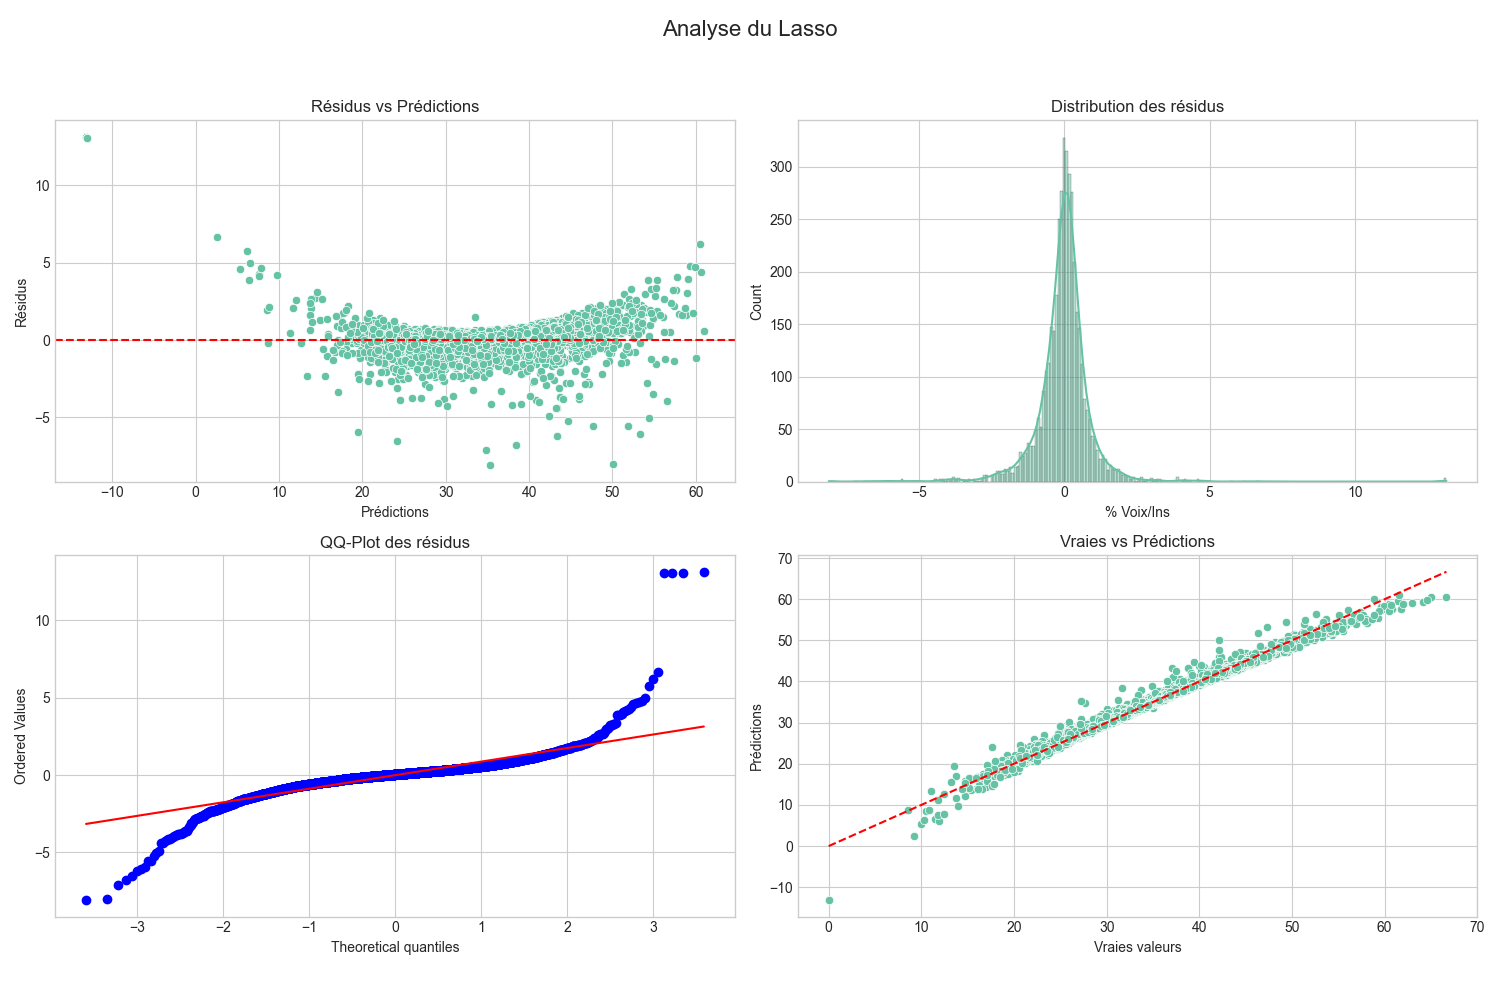
\includegraphics[width=0.8\textwidth]{figures/graphs_analyse_model_Lasso.png}
        \end{center}
    
    \end{frame} 

              
        
    \begin{frame}{XGBoost}
        \begin{center}
            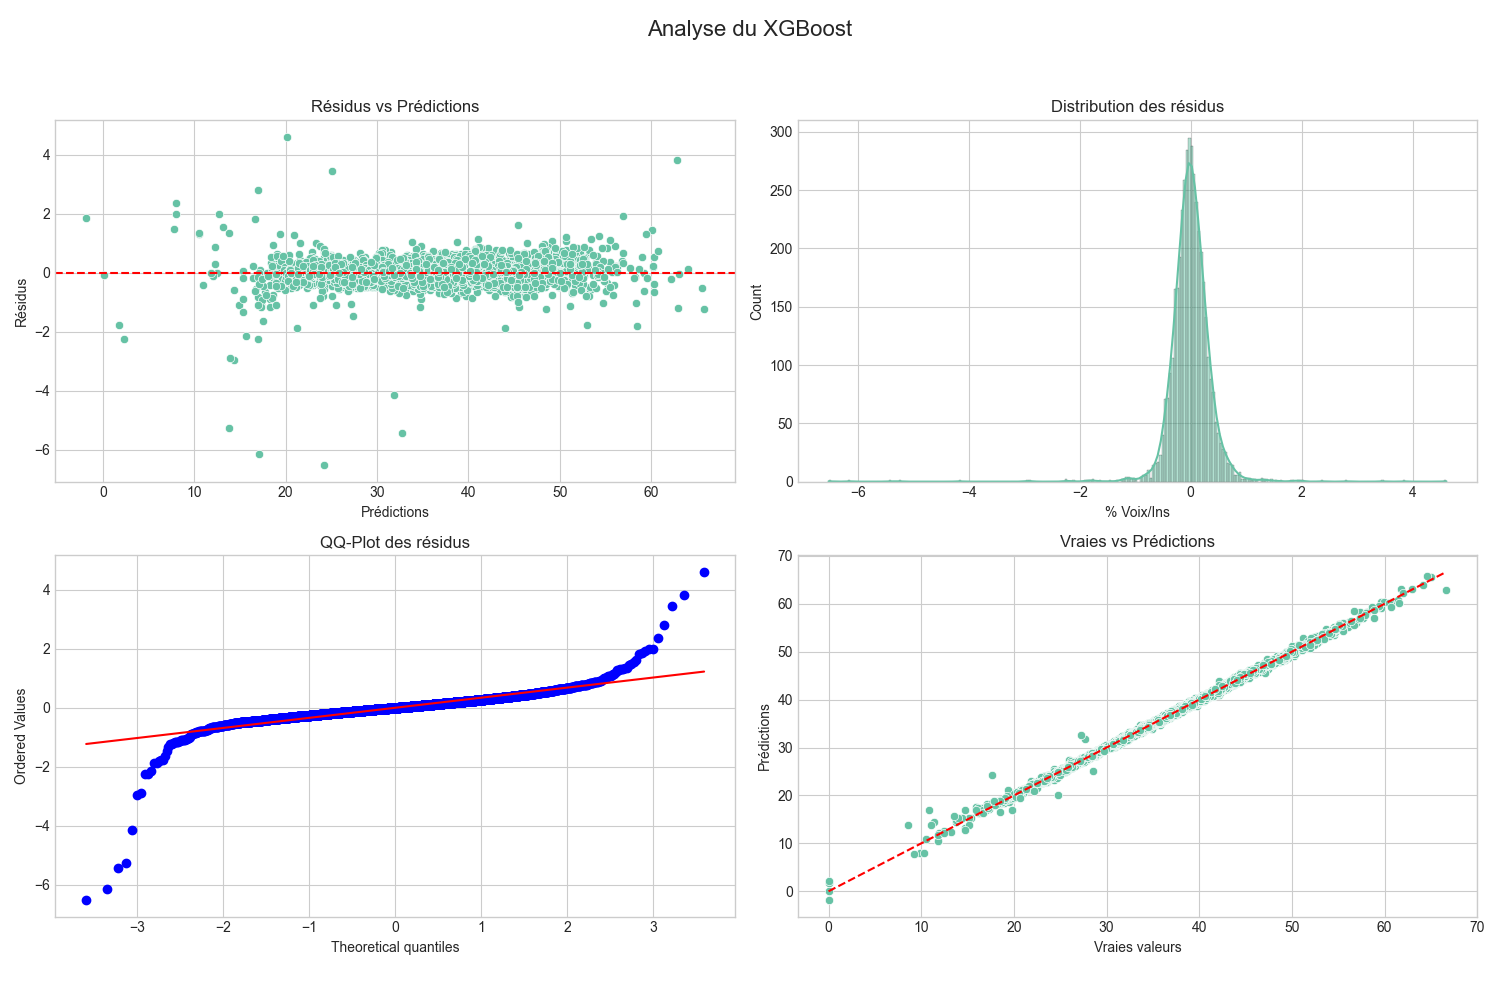
\includegraphics[width=0.8\textwidth]{figures/graphs_analyse_model_XGBoost.png}
        \end{center}
    
    \end{frame}    
        


\begin{frame}[allowframebreaks]{Interprétation des graphiques}
    
    les QQ-plots des résidus :  vus qu'ils représentent les quantiles d'une distribution normale théorique vs ceux observés , et comme les deux modèles ont des courbes en 'S' très applaties et presque centrée sur la diagonale , ont en conclut que 'les résidus des deux modèles on une distribution  presque normale '
                
    \framebreak        
    Histogrames des résidus : la différence notable , ce sont l'intervalles sur lesquels ils s'étalent :
        \begin{itemize}
            \item[.] ceux de XGBoost s'étalent de -6 à 6
            \item[.] ceux de Lasso s'étalent de -11 à 11
        \end{itemize}

        cela veut dire que les erreurs de Lasso varient beaucoup (prennent des valeurs plus ) plus que ceux de XGBoost , donc XGBoost est préférable comme modèle

    \framebreak

    \textbf{ Residus vs Prédictions} : les graphiques montres que les residus de XGBoost sont plus concentrés autour de zero que ceux de Lasso . On ve
    
    \framebreak

    \textbf{}
\end{frame}


\subsection{Importance des features}
\begin{frame}[allowframebreaks]
\frametitle{Les meilleurs features pour Lasso}
    un premier truc

    \framebreak
\end{frame}





\clearpage
\pagenumbering{roman}



\end{document}
